
\chapter{Results}
The culminating part of this nuclear physics analysis begins with the extraction of the experimentally measured DIS cross sections for three targets. Then using those cross sections to study the per nucleon scaled A/D ratio. I will also use these A/D ratios to study the EMC effect for both helium-3 and tritium. In this chapter, I will present my results for the DIS cross sections and EMC effect. I will also discuss an error analysis for both the cross section measurements and the EMC effect results. 
\section{DIS Cross Section}
\paragraph{}Using the Monte Carlo ratio method, I extracted the experimental measured cross section for helium-3, tritium, and deuterium. These DIS cross section extraction ranges from 0.18 to 0.82 in $x$, from 2.2 to 11.8 GeV$^2$ in $Q^2$, and has W$^2$ $>3.5$ GeV$^2$. The central momentum setting of the spectrometer was 3.1 GeV/c and the spectrometer was moved from 17.5 to 33.5 degrees.


\begin{equation}
\sigma_{Data} = \sigma_{model} \cdot \frac{Y_{Data}}{Y_{MC}}. \nonumber
\end{equation}
%\begin{landscape}
%\begin{sidewaysfigure}
\begin{figure}
%	\hspace{-80pt}
	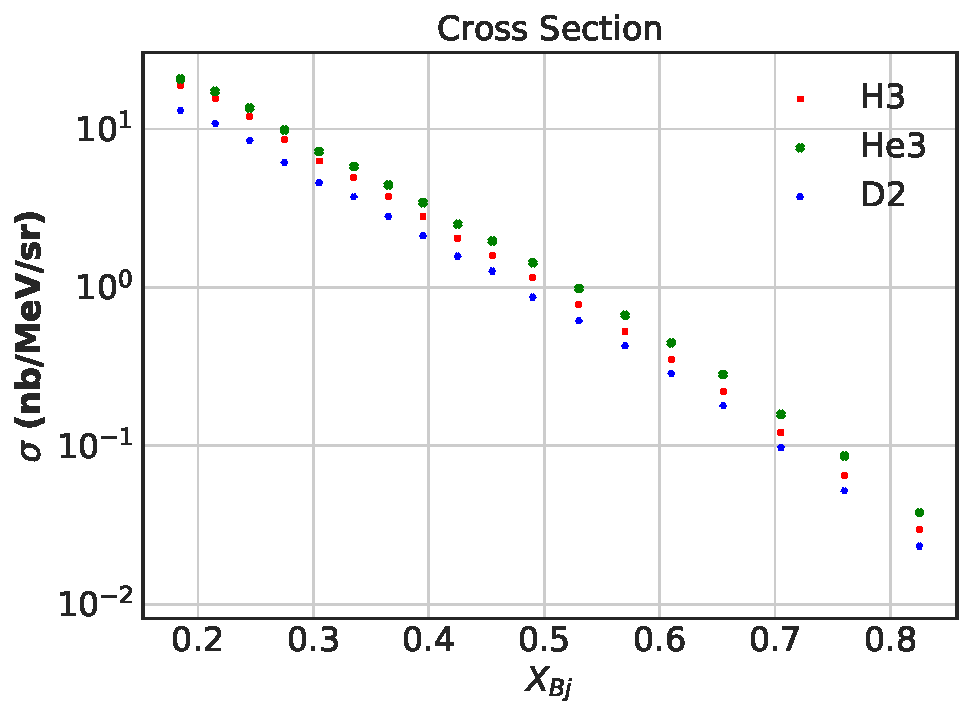
\includegraphics[width=15.5cm]{../images/total_xs.pdf}
	\caption{Experimentally measured cross section using the Monte Carlo ratio method for tritium, helium-3, and deuterium. Normalization uncertainty due to target thickness uncertainty for tritium= 0.97\%, helium-3 = 1.12\%, and deuterium = 0.56\%.}
    \label{CCplot}
\end{figure}
%\end{sidewaysfigure}
%\end{landscape}
I compared the data yield to the Monte Carlo yield to produce a correcting factor for the model cross section. Figure \ref{D_MC_COMP} shows the ratio comparison between data and Monte Carlo in bins of $x$. Then apply the ratio factor for a bin in $x$ to the model cross section to extract out the experimentally measured cross section for that bin. Figure \ref{CCplot} shows a plot of the experientially measured cross section for tritium, helium-3, and deuterium.  This is the first result of an inclusive DIS cross section for tritium.  Appendix (?) contains a table of the cross section and summaries of the errors included in the error study for the cross section analysis. 
\section{Cross Section Error Analysis}
The measurement of the cross section requires finally tune detectors and analysis process. Uncertainties arise due to the nature and limitations of the spectrometers and the analysis of the data received. In this section, I will discuss the calculation and propagation of errors in the analysis of the DIS cross section. The error analysis will be broken into the calculation of normalized yield for data, yield for Monte Carlo, and the cross section extraction. 

\begin{table}[]
	\caption{Relative Error Contributions in $\%$ for Cross Section for a selection of bins. This table contains the summary of relative error to the cross section for the yield, Monte Carlo, and Cross Section Model.}
	\centering
	\begin{tabular}{|l|l|l|l|}
		\hline
		\textbf{\qquad \qquad\qquad x bin}   & \textbf{0.215} & \textbf{0.455} & \textbf{0.705} \\ \hline\hline
		Statistical             & 0.512 & 0.889 & 1.106 \\ \hline
		Efficiency Error*       & 0.665 & 1.477 & 2.951 \\ \hline
		Positron Correction     & 0.036 & 0.016 & 0.005 \\ \hline
		End cap Correction     & 1.0 & 1.0 & 1.0 \\ \hline
		Charge Calculation     & 0.2 & 0.2 & 0.2 \\ \hline
		Density Correction      & 0.2 & 0.2 & 0.2 \\ \hline
		Monte Carlo Statistical & 0.193 & 0.217 & 0.209 \\ \hline
		Optics Reconstruction	& ?0.665& ?1.477 &?2.951 \\ \hline
		??Cross Section Model 	& ?0.193 & ?0.217 & ?0.209 \\ \hline
		??Radiative Corrections\cite{primer} 	& 0.5  & 0.5 & 0.5 \\ \hline
		Total Error		 	 	& 0.95  & 1.931 & 3.316 \\ \hline
	\end{tabular}
\end{table}

\begin{align}
\dfrac{d\sigma}{dE^{\prime}d\Omega} &= \frac{(N - BG)}{\mathscr{L} \cdot \epsilon \cdot \Delta E^{\prime} \Delta \Omega \cdot A(E^{\prime},\theta)}. \nonumber\\
\sigma &= \text{NormY}/\left(\Delta E^{\prime} \Delta \Omega \cdot A(E^{\prime},\theta)\right)\nonumber\\
\text{NormY} &= \left(N_e \cdot BG/\epsilon \right) / \mathscr{L}
\end{align}
\subsection{Normalized Yield Error}
\subsubsection{Corrected Electron Count Error}
\paragraph{}
The contributions for error on the measurement of the normalized yield(normY) can be simplified into the contributions for the corrected number of electrons and the luminosity. The error for the corrected number of counted electrons includes the random statistical error for the count of electrons detected, the error associated with the calculated efficiencies, and the error from the background correction. The electron statics range from 4875 to more then 42000 in a bin and therefor I have treated the randomness of the counting in a standard error technique. The relative statistical error for a bin is $\frac{1}{\sqrt{Ne}}$ and ranges from .5\% to 1.4\%. Calculating the efficiencies deals with calculating a probability of a binomial choice. The errors associated with the efficiencies are calculated using the Wilson score interval described in equation \ref{WSI}, where $p$ is the efficiency or a probability of a success, $n$ is the number of samples, $z$ is 1.645 for a 95\% confidence level. 
\begin{equation}
p[_{UpperBound},_{LowerBound}] = \frac{ 2np +z^2 \pm \left[z\sqrt{z^2 - \frac{1}{n} + 4np(1-p) +(4p-2)} + 1 \right]}{2(n+z^2)} \label{WSI}
\end{equation}
The relative efficiency errors are added in quadrature to calculate an over all efficiency error to be propagated into the yield calculation.
\paragraph{}The correction for background events corrects for events from the end caps and pair produced electrons. The end cap correction factor is produced by a ratio of yields between the gas cells and the empty cell. This yield measurement allows for the cancellation of many of the systematic uncertainties. The largest contribution to the this error is the low statistics of the back ground events. The estimated error to the cross section analysis is about 1\%. Furtherer study of the end cap contamination and the error associated with the correct is part of the ongoing analysis. The error for the positron correction involves using the covariance matrix for the exponential fit and propagating the error for each parameter of each target using the $x_{Bj}$ dependent function. The error for the fit parameters are propagated to an error for the correction using equation \ref{cv_err}.
\begin{equation}
\frac{\Delta f(x)}{f(x)} =  \sqrt{ \sum_{i}^{} \left(\delta p_i\cdot x^i\right)^2 + \sum_{ij}^{}\left( 2\cdot \delta p_{ij}\cdot \dfrac{df(x)}{dp_i}\cdot \dfrac{df(x)}{dp_i}\right) } \label{cv_err}
\end{equation}
The error for the background corrections are added in quadrature to get an overall error for the total back ground correction.  
\subsubsection{Luminosity Error}
\paragraph{}The errors involved in the luminosity calculated is the target density thickness measurement, beam charge calculation, and density correction. The error in the target thickness measurement is considered a overall normalization uncertainty. The error for the three gas targets' thickness measurements are: tritium= 0.97\%, helium-3 = 1.12\%, and deuterium = 0.56\% \cite{HATT_eng}. The measurement uncertainties for each gas target are displayed in table \ref{tgt_table}. The amount of beam charge deposited on the target is calculated via the BCM(beam charge monitors) and their calibrations. The BCM calibrations were determined a few times through the run period with no change to the calibration constants. Due to the consistency of the BCMs and the high quality calibration the  error estimation for charge calculation is approximately 0.2\%. The error for the density correction is based in the error from the 2nd order polynomial fit. The error is calculated using the same method as the positron background correct, combining the errors for the fit parameters and the covariance terms through the propagation formula \ref{cv_err} using the current dependent correction function, \ref{eq:dc}. The relative error in charge on target and density correction have been added in quadrature to calculate a systematic error for the luminosity calculation. The systematic error for the luminosity and the systematic error for the correct count of electrons are then added in quadrature to calculate and overall normalized yield error.  
\subsection{Monte Carlo Yield Error}
\paragraph{}The responsibility of the Monte Carlo is to accurately account for the acceptance of the spectrometers. The uncertainty for thee Monte Carlo yield combines the statical uncertainty of the number of events generated and the reconstruction of the momentum and angle.  The statistical uncertainty is reduced due to the generation of a few million events. The uncertainty in the reconstruction of an event is a mixture of the uncertainties in the beam x and y position, spectrometer offsets, beam energy, optics, and acceptance cuts. The uncertainties for the beam x and y position was controlled by the BPMs and the calibration I completed. The uncertainty for the BPM measurements is 140 $\mu$m. The beam energy measurement is quoted to have an absolute accuracy of 5 x 10$^{-4}$.  The optics are capable of determining the relative in-plane angle with an accuracy of $\pm$ 0.2 mrad, out-of-plane angle with $\pm$ 0.6 mrad in the target coordinates, and momentum reconstruction 2.5x10$^{-4}$\cite{HallA}.  Using equation \ref{scatangle}, I propagated the resolution of target reconstruction variables to determine the relative uncertainty of the scattered angle to be $\approx$ 0.15\%. I have calculated the effect of the accuracy of the optics by comparing the cross section for the nominal values of , beam energy, scattered angle, and momentum, to the cross section of these values shifted by their uncertainties. A summary of the uncertainties used in the uncertainty of optics reconstruction are listed below.
\begin{itemize}
\item$\delta \theta$ = 0.15\%
\item$\delta E^{\prime}$ = $\pm$0.00025
\item$\delta E_{beam}$ = $\pm$0.0005
\end{itemize}
Using the errors in scattering angle, scattering momentum, and beam energy, I calculated an approximate error associated with the reconstruction events into $x$ bins with equation \ref{reconErr}. The fluctuation of this error is large and ranges from 1/2\% to 1.5\% and therefor will be applied on a point to point bases. 

\begin{equation}
\frac{\Delta \sigma(E,E^{\prime},\theta)}{ \sigma(E,E^{\prime},\theta)} = \frac{\sigma(E+\Delta E_{beam},E^{\prime}+\Delta E^{\prime},\theta+\Delta \theta) - \sigma(E,E^{\prime},\theta)}{\sigma(E,E^{\prime},\theta)} \label{reconErr}
\end{equation}

\subsection{Cross Section Model Error}
\paragraph{}
The model dependence of the DIS cross section and the radiative corrections are the two factors of the systematic error that accompanies the Monte Carlo ratio method. My analysis of the model depended errors used different DIS cross section models to supply an error for the model cross section and the radiative corrections. The models I will used to study the model dependent error can be broken into 3 sections, models for F$_{2d}$, model for EMC correction, and model for the ratio for $F_{2n}/F_{2p}$. I will two models to form the deuterium structure function Ari Bodek \cite{DISmodel} and M. Arneodo's NMC model \cite{NMC_model}. I will use two EMC correction models, Kulagin, S. A. and Petti, R. \cite{kpmodel}, and a SLAC EMC correction \cite{SLAC_bodek}. The structure function ratio is formed by two models also, linear Ratio = (1 - 0.8$*x$) and NMC \cite{NMC_ratio}. The model depended error was estimated by comparing the different models together with the chosen model. In the extreme case, this error reached a maximum of 2\%    

\section{EMC Ratios}
\paragraph{}In this section, I will present the A/D cross section ratios for helium-3 and tritium. The ratios are normalized by the number of nucleons in each target. Included in figure \ref{ADplot} are results from E03103. These results have different invariant mass but are considered DIS until 0.65 in $x$. Above this threshold, the invariant mass begins to drop lower then the DIS criteria used for my analysis. 
%\begin{landscape}
%\begin{sidewaysfigure}
%\thispagestyle{empty}
%\raisebox{-14.5cm}{\makebox[\linewidth]{\thepage}}
\begin{figure}
	\centering
	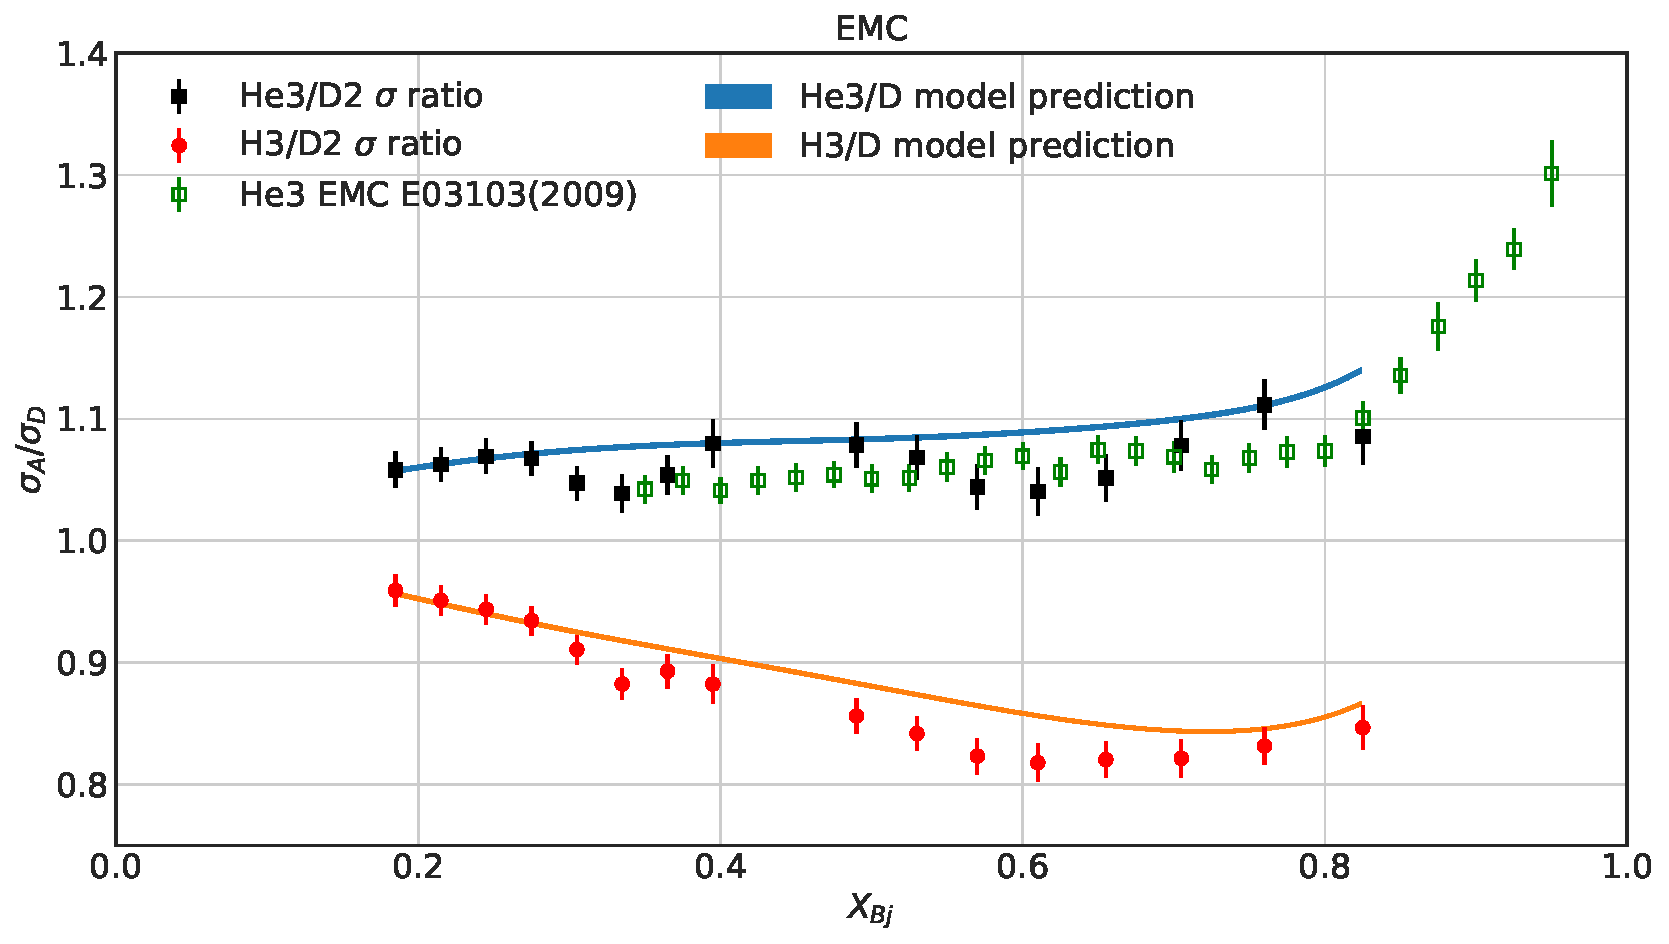
\includegraphics[width=15.5cm]{../images/A_D_ratios.pdf}
	\caption{The A/D ratio for helium-3 and tritium from my analysis. Also included, EMC analysis from E03103\cite{seeley} and the EMC ratios from a DIS scattering model from Arie Bodek model \cite{DISmodel}.}
	\label{ADplot}
\end{figure}

%\end{sidewaysfigure}
%\end{landscape}

\subsection{Isoscalar Correction}
	\paragraph{}The definition of an EMC effect ratio is the ratio of the per nucleon cross section ratio of a target nucleus with deuterium. Also,  this comparison is of a target with equal number of protons and neutrons, an isoscalar nuclei. When looking at the EMC ratio of a target with not an equal number of nucleons, an isoscalar correction needs to be applied. This correction is used to correct for the difference in cross section between the neutron and proton. The per nucleon nuclear F$_2^A $ of an unsymmetrical nucleon can be written as:
	\begin{equation}
	\frac{1}{A}\left(ZF^p_2 + \left(A-Z\right)F^2_n\right)\nonumber
	\end{equation}
	and a symmetrical nucleon can be simplified to:
	\begin{equation}
		\frac{1}{2}\left(F^p_2 + F^2_n\right).\nonumber
	\end{equation}	
	The isoscalar correction can be determine by applying a correction function $f_{iso}$ to equate the two previous equations and solving that combination for the correction function.
	\begin{equation}
		\frac{1}{2}\left(F^p_2 + F^2_n\right) =  f^A_{iso}\frac{1}{A}\left(ZF^p_2 + \left(A-Z\right)F^2_n\right)\nonumber
	\end{equation}
	\begin{equation}
	f^A_{iso} = \frac{\frac{1}{2}\left(1+F^n_2/F^p_n\right)}{\frac{1}{A}\left(Z +(A-Z)F^n_2/F^p_n\right)} \label{isoC}
	\end{equation}
	\paragraph{}The isoscalar correction for a nuclear target depends on A,Z, and the F$_2$ ratio. There exist no data on the free neutron, so the $F^n_2/F^p_n$ is a model dependent extraction. The  F$_2$ ratio has been extracted from the ratio of tritium to helium from the MARATHON experiment and deuterium to hydrogen ratios from previous experiments from SLAC and the NMC. I have used the $F^n_2/F^p_n$ from MARATHON to calculate my iscscalar correction for both helium-3 and tritium. I have estimated the error of this model dependent correction by comparing the isoscalar correction from the MARATHON extraction with the isoscalar correction using three other $F^n_2/F^p_n$ models Kulagin, S. A. and Petti, R. \cite{kpmodel}, J. Arrington \cite{JA_FR}, and NMC \cite{NMC_ratio}. The relative variance of this calculation ranges from $\pm$ 0.1\% to $\pm$ 3.8\% for tritium EMC ratio. These 4 models and the error band from this study is shown in figure \ref{isofuncs}.

	\begin{figure}[t]
		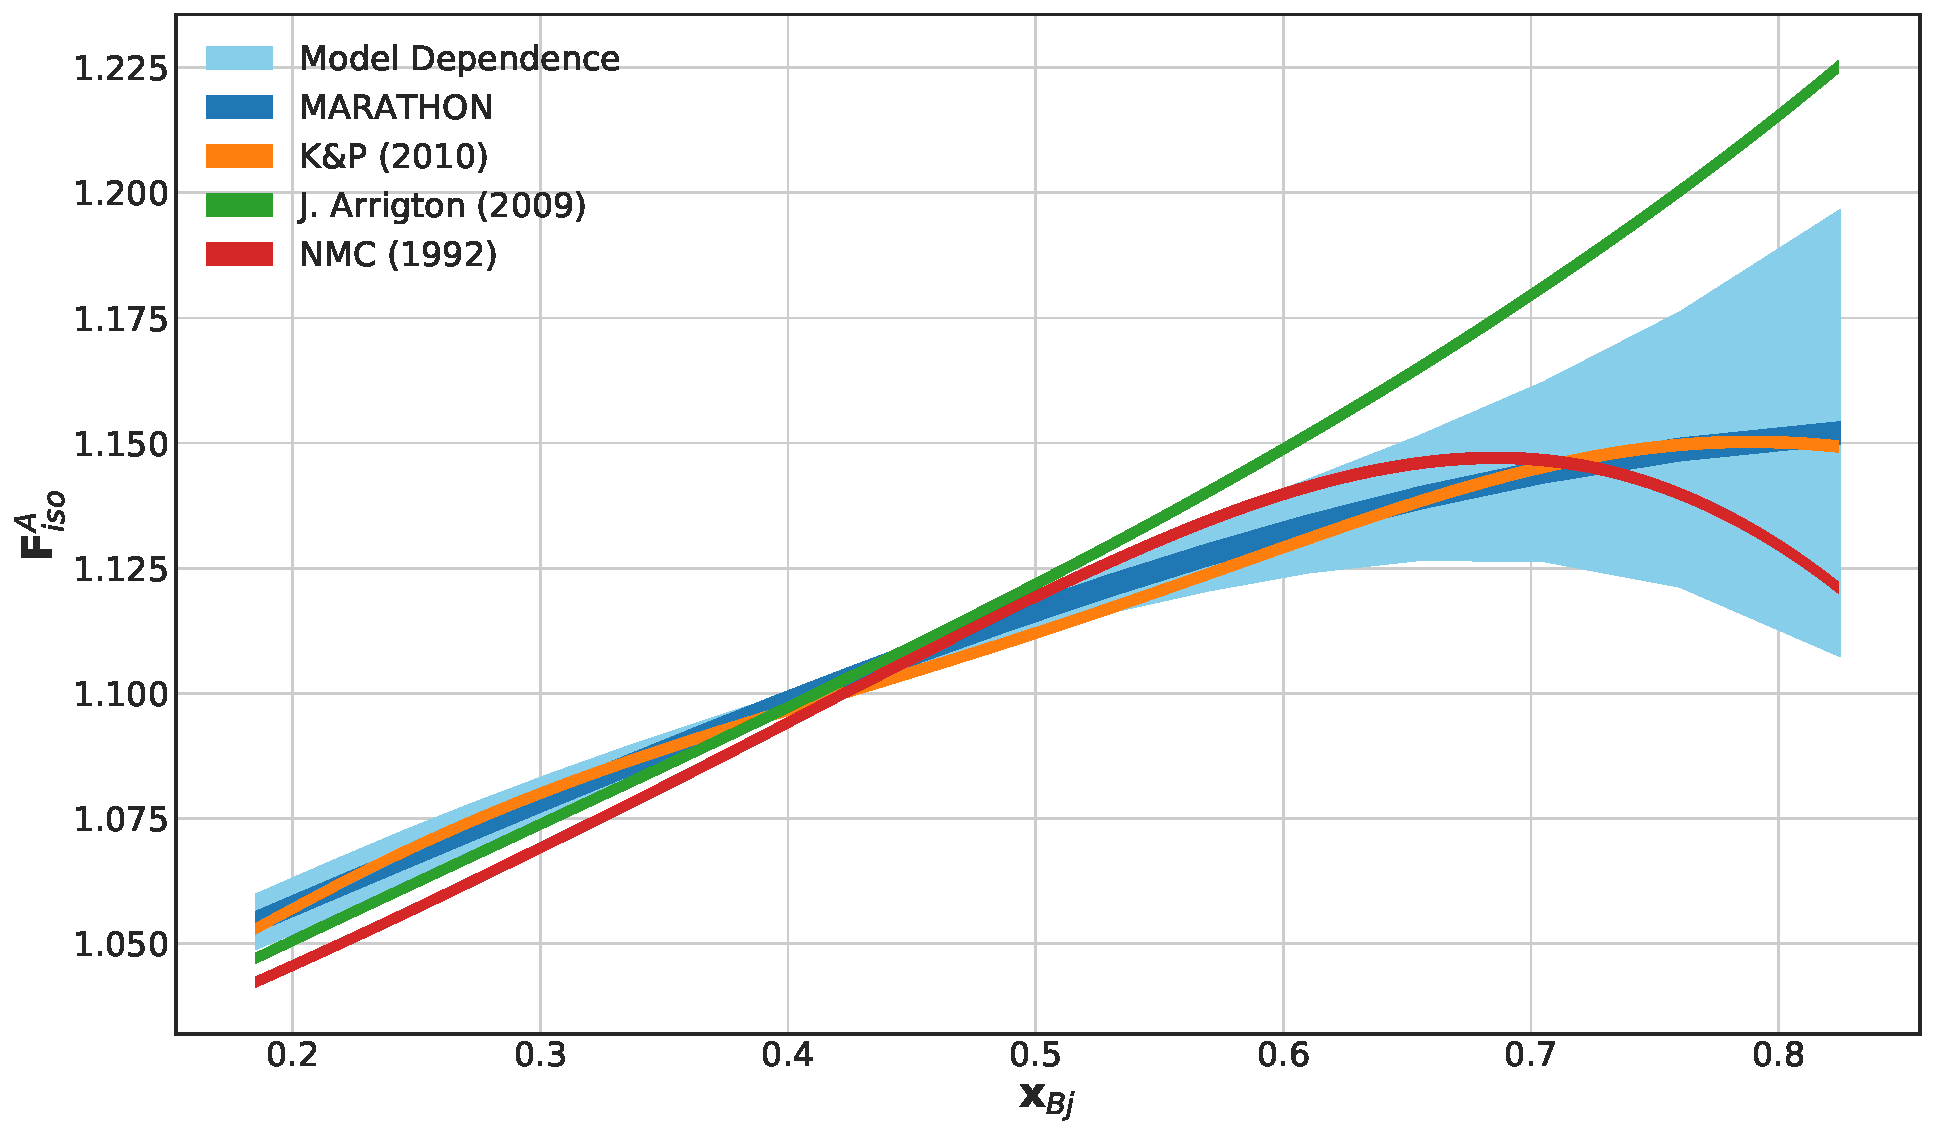
\includegraphics[width=15cm]{ISOfacsH3.pdf}
		\caption{Isoscalar correction factor for the tritium EMC ratio from four different models discussed in this section.}
		\label{isofuncs}
	\end{figure}
	\begin{figure}
		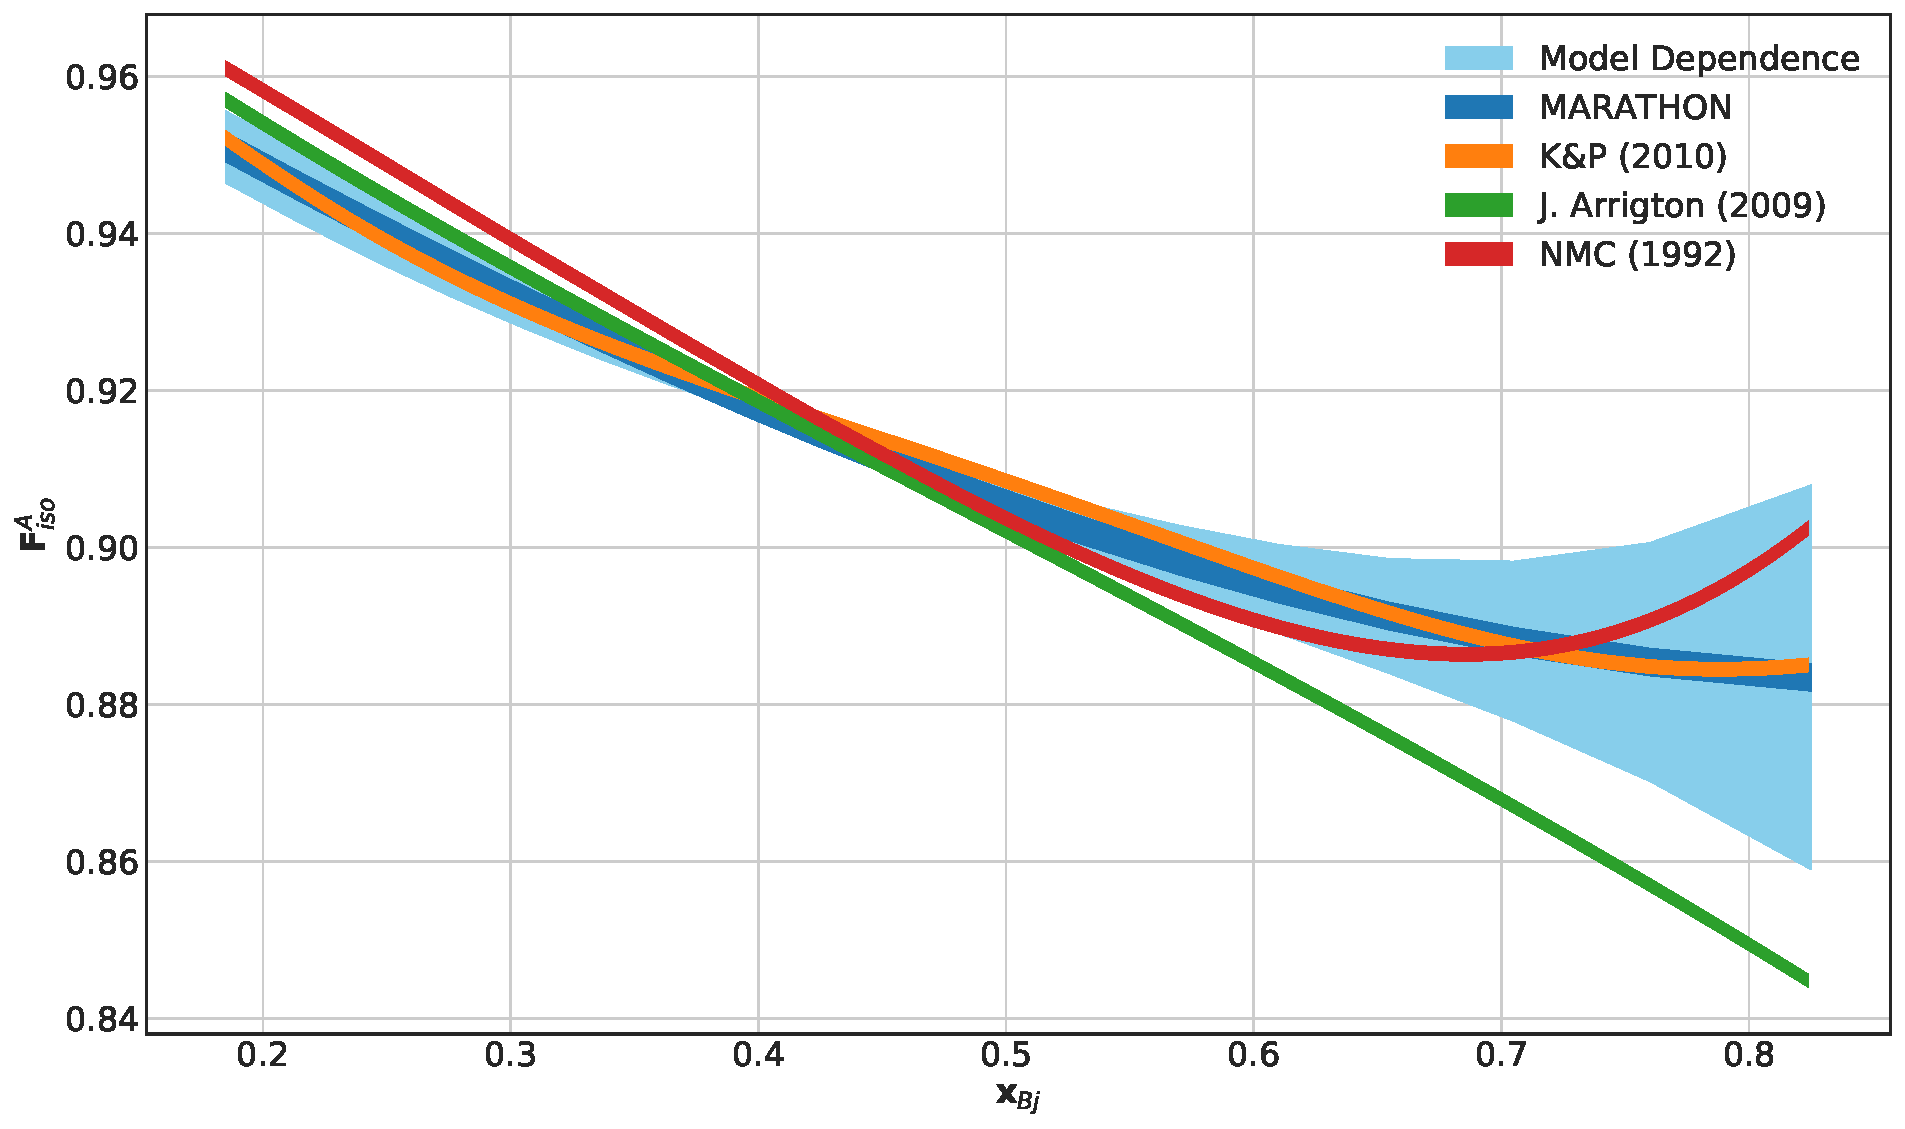
\includegraphics[width=15cm]{ISOfacsHe3.pdf}
		\caption{Isoscalar correction factor for the helium-3 EMC ratio from four different models discussed in this section.}
		\label{isofuncsHe3}
	\end{figure}

\section{EMC Effect}
\paragraph{} The MARATHON experiment was designed to study the ratio of yields between nuclear targets. The process of studying ratios help eliminate many systematic errors. MARATHON's design of rotating targets, and uniform data taking procedure allows the cancellation of the detector efficiency correction facto and corrections due to acceptance issues. This will reduce the size of the uncertainty of the EMC effect measurement and provides a better result for the EMC ratio of the two A=3 nuclei. The isoscalar corrected EMC Effect ratios for helium-3 and tritium from my inclusive DIS cross section extraction are displayed in figure \ref{ISOEMC_B}.   

	\begin{figure}
		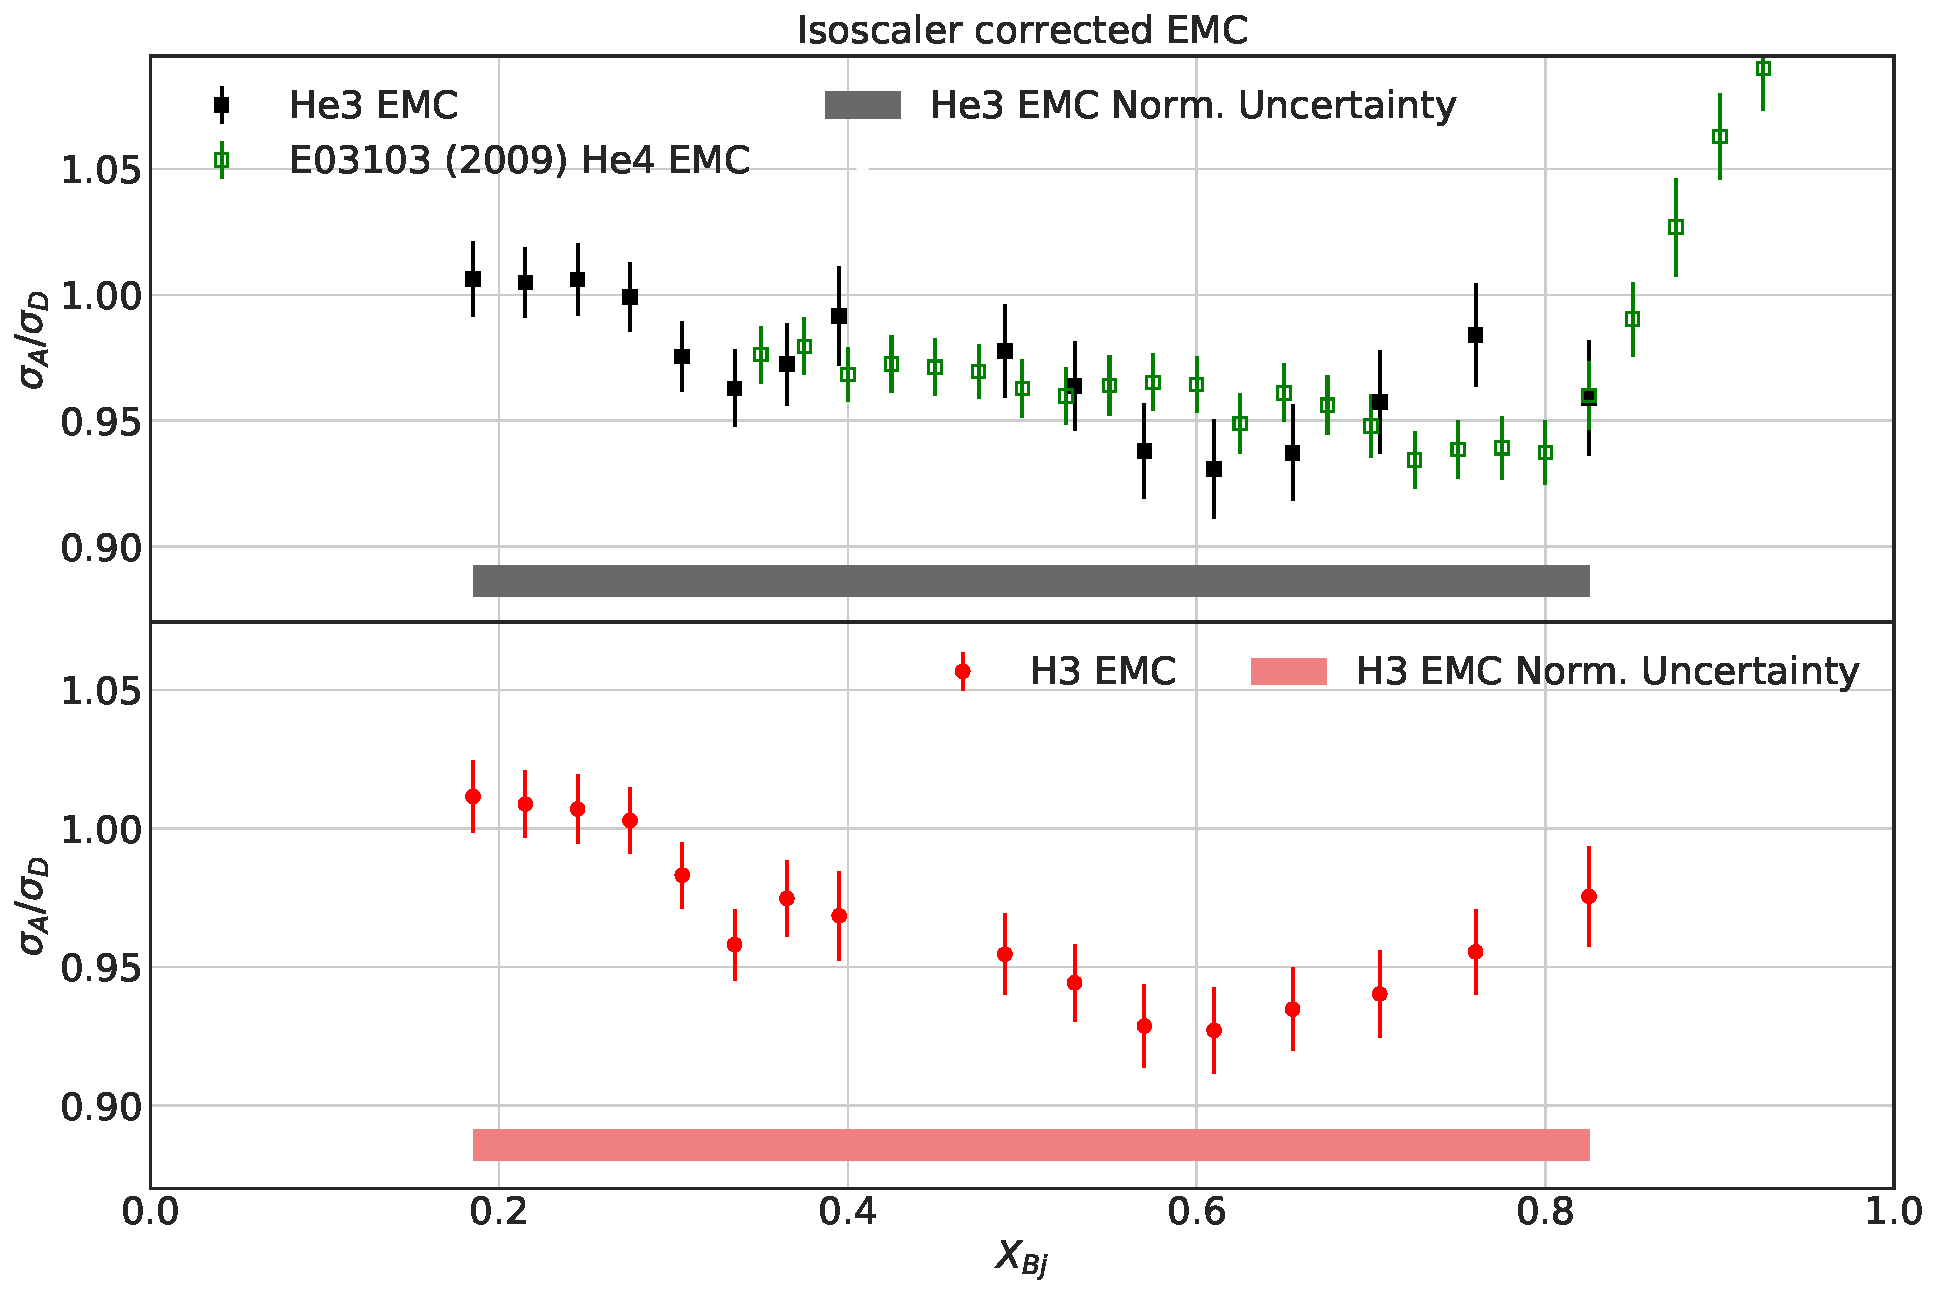
\includegraphics[width=15cm]{EMCIsotwo.pdf}
		\caption{Isoscalar correction factor for the helium-3 EMC ratio from four different models discussed in this section.}
		\label{ISOEMC_B}
	\end{figure}